\documentclass[margin,line]{CV}

\usepackage{graphicx}
\usepackage{wrapfig}
\usepackage{ifthen}
\usepackage{url}

\newboolean{foreign}
\setboolean{foreign}{false}

\begin{document}
\name{\Large Fokin Aleksandr}
\begin{resume}

\begin{wrapfigure}{r}{2cm}
    \vspace{-20pt}
    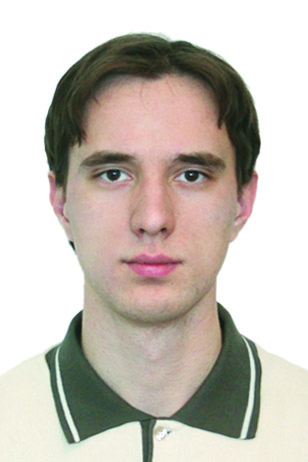
\includegraphics[width=2cm]{photo.jpg}
    \vspace{-20pt}
\end{wrapfigure}

    \section{\mysidestyle Contact\\Information}
    Current Location: Los Angeles, United States \\
    \\
    Mobile: 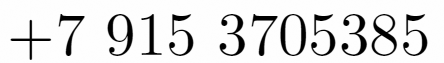
\includegraphics[height=0.35cm]{phone.png} \\ 
    E-mail: apfokin@gmail.com \\
    \\
    \\

    \section{\mysidestyle Education}
    \textbf{Faculty of Computational Mathematics and Cybernetics, Moscow State University}, Moscow, Russia \vspace{2mm}\\\vspace{1mm}%
    \textsl{\ifthenelse{\boolean{foreign}}{Bachelor's}{Specialist} degree in Applied Mathematics and Computer Science} \hfill \textbf{September 2004 - July 2009}\vspace{1mm}\\
    Advisor: Professor Chernov Alexander \\
    Thesis: Reconstruction of Class Hierarchies for Decompilation of C++ Programs \\
    I have graduated with high honors. Diploma GPA is 5.0 out of 5.0.

    \textbf{Graduate School of Science and Engineering, Chuo University}, Tokyo, Japan \vspace{2mm}\\\vspace{1mm}%
    \textsl{Full-time non-degree student} \hfill \textbf{September 2008 - March 2009}\vspace{1mm}\\
    Advisor: Professor Mitsunori Makino \\
	I was studying Japanese, working on algorithms for real-time ray tracing and have implemented a real-time ray tracer for use with CAVE automatic virtual environment.

    \section{\mysidestyle Research\\Interests}
    Image-based modeling and rendering, 3d reconstruction.
    Ray tracing and global illumination, especially in real time.
    Software reverse engineering, binary translation, decompilation.

    \section{\mysidestyle Research\\Experience}
    \textbf{Institute for System Programming of the Russian Academy of Sciences} \vspace{2mm}\\\vspace{1mm}%
    \hfill \textbf{July 2008 - September 2010}\\
    I was doing research on decompilation of C++ programs.

    \textbf{Select LTD} \vspace{2mm}\\\vspace{1mm}%
    \hfill \textbf{October 2010 - September 2011}\\
    I continued C++ decompilation research at Select LTD.

    \section{\mysidestyle Publications}
    A. Fokin, E. Derevenetc, A. Chernov and K. Troshina. ``SmartDec: Approaching C++ Decompilation'',
	in proceedings of the \textsl{18th Working Conference on Reverse Engineering}, pp. 347-356, 2011.
	
	A. Fokin, K. Troshina and A. Chernov. ``Reconstruction of Class Hierarchies for Decompilation of C++ Programs'',
    in proceedings of the \textsl{14th European Conference on Software Maintenance and Reengineering}, pp. 249-252, 2010.

    K. Troshina, A. Chernov and A. Fokin. ``Profile-Based Type Reconstruction for Decompilation'',
    in proceedings of the \textsl{17th International Conference on Program Comprehension}, pp. 263-267, 2009.

    \pagebreak

    \section{\mysidestyle Professional\\Experience}
    \textbf{Intel Student Research Lab at the Moscow State University} \vspace{2mm}\\\vspace{1mm}%
    \textsl{Software Developer} \hfill \textbf{February 2007 - April 2008}\\
    I have implemented a panorama stitching application in C++. I was subsequently offered an intern position 
	at Intel but had to turn it down due to personal reasons.

    \textbf{Institute for System Programming of the Russian Academy of Sciences} \vspace{2mm}\\\vspace{1mm}%
    \textsl{Software Developer} \hfill \textbf{September 2007 - September 2008}\\
    I was working as a C++ programmer in a team developing a framework for dynamic analysis of binary code.
	Using C++ metaprogramming techniques I have implemented a disassembler for MIPS64 architecture that 
	outperformed all other disassemblers for this architecture known to our team.

    \textbf{Select LTD} \vspace{2mm}\\\vspace{1mm}%
    \textsl{Software Developer} \hfill \textbf{July 2009 - September 2011}\\
    I have written some parts of the backend for \url{http://mathege.ru} and have implemented a form recognition system
    that is currently used in some of the Moscow schools for exam results checking. Detailed description of the system is
    available at \url{http://elric.ru/wordpress/projects/form-recognition-toolkit/}. 
	
	I was also a lead developer of the SmartDec native code decompiler. Detailed description is available at 
	\url{http://decompilation.info}.

	\textbf{Combild LLC} \vspace{2mm}\\\vspace{1mm}%
	\textsl{Software Development Lead, Co-founder} \hfill \textbf{June 2010 - December 2011}\\
    I was working on a program complex for IT infrastructure management that targeted small companies and IT outsourcers. I was responsible for the overall product architecture and was managing a small development team. After a year of development we have secured our first customers, but at that point the cash inflow we had wasn't sufficient to cover our expenses. Unable to secure the funding, we had to close the project.

    \textbf{Network Optix, Inc.} \vspace{2mm}\\\vspace{1mm}%
    \textsl{Senior Software Developer} \hfill \textbf{October 2011 - present}\\
    I'm currently working on HD Witness, an Enterprise Video Management System (VMS). 
    
    For the initial release I have almost single-handedly implemented the client application that was very well received in the industry. Various sources have described HD Witness as the most visually appealing and user-friendly VMS on the market. 
    
    Currently my main responsibilities include ensuring UI and UX performance and consistency of our desktop and mobile clients, management of the front-end development team, design of public APIs and development of generic C++ libraries that are used internally.
    
	\textbf{Personal Projects} \vspace{2mm}\\\vspace{1mm}%
	Some of my personal and freelance projects are listed on my website: \url{http://elric.ru/wordpress/projects}.

    \pagebreak
    
    \section{\mysidestyle Honours and\\Awards}
    7th Moscow Collegiate Programming Contest, 11th place, Moscow, 2005.                            \vspace{1mm}\\%
    8th Moscow Collegiate Programming Contest, 9th place, Moscow, 2006.                             \vspace{1mm}\\%
    M.V. Lomonosov Scholarship for Academic Excellence, Moscow, 2006-2009.


    \section{\mysidestyle Related\\Skills}
    Substantial experience with C++ and Java. \\
	Deep understanding of the underlying principles of modern C++ libraries and frameworks such as Qt and boost. \\
    A lot of experience writing cross-platform C++ code. \\
    Considerable experience with multithreading in C++ and Java. \\
    Knowledge of modern realtime rendering techniques and APIs. \\
    Proficiency in UX and UI design and implementation. \\
    Experience with Delphi, x86 Assembly, Linux shell scripting, SQL. \\
    Some experience with C\#, Matlab, Perl and Python. \\


    \section{\mysidestyle Languages}
    Russian: native \\
    English: fluent \\
    Japanese: intermediate


    \section{\mysidestyle References}
    {\sl Available upon request.}

\end{resume}
\end{document}



















